% \begin{abstract}

%     \acrfull{csacs} can be considered as one of the most significant advancements in timekeeping technology given their low power consumption, small size, and high precision.
%     Originally developed for military purposes, \acrshort{csacs} have found applications in various fields where accurate timekeeping and portability are essentials, such as satellite navigation, telecommunications, and space exploration.

%     This report will provide an overview of the key parameters defining their performance, discuss the governing physics highlighting the bottleneck and limitations, and explore their current and potential applications across different sectors.
%     A final section will highlight the future prospects and challenges in the development of \acrshort{csac} technology.

% \end{abstract}

\section*{Abstract}

\acrfull{csacs} can be considered as one of the most significant advancements in timekeeping technology considering their low power consumption, small size, and high stability and accuracy in frequency.
Originally developed for military purposes, \acrshort{csacs} have found applications in various fields where accurate timekeeping and portability are essentials, such as satellite navigation, oil industry exploration, telecommunications, and space experimental physics.

This report will provide an overview of the key parameters, discuss the governing physics highlighting the bottleneck and limitations, and explore their current and potential applications across different sectors.
A final section will focus on the future prospects and challenges in the development of the next generation of \acrshort{csac} technology.

\vspace{1cm}

\begin{figure}[H]
    \centering
    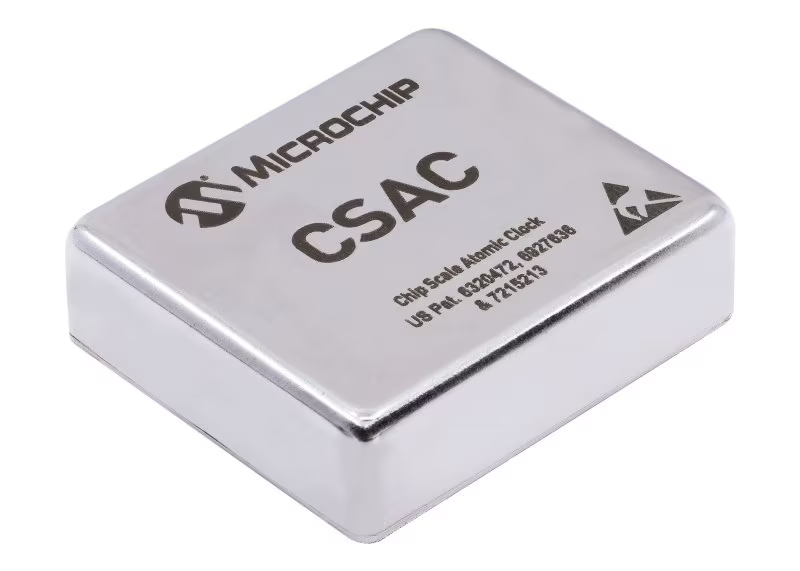
\includegraphics[width=.6\textwidth, max width=.8\linewidth]{img/microsemi-SA65.png}
    \caption{
        Microsemi SA.65 Chip Scale Atomic Clock, the most advanced \acrshort{csac} commercially available since 2021.
        Source: \cite{MICROCHIP}.
    }
    \label{fig:microsemi_SA65}
\end{figure}